\documentclass[border=10pt]{standalone}
\usepackage{tikz}
\usetikzlibrary{arrows.meta, positioning, calc, fit, backgrounds, decorations.pathreplacing,
    patterns}
\usepackage{xcolor}
\usepackage{amsmath}

% Brand colors
\definecolor{Garnet}{HTML}{73000A}
\definecolor{Atlantic}{HTML}{466A9F}
\definecolor{Congaree}{HTML}{1F414D}
\definecolor{Horseshoe}{HTML}{65780B}
\definecolor{Rose}{HTML}{CC2E40}
\definecolor{Honeycomb}{HTML}{A49137}
\definecolor{LightGray}{HTML}{ECECEC}
\definecolor{Black90}{HTML}{363636}
\definecolor{Black70}{HTML}{5C5C5C}
\definecolor{Black50}{HTML}{A2A2A2}
\definecolor{Black30}{HTML}{C7C7C7}
\definecolor{WarmGrey}{HTML}{676156}

\begin{document}
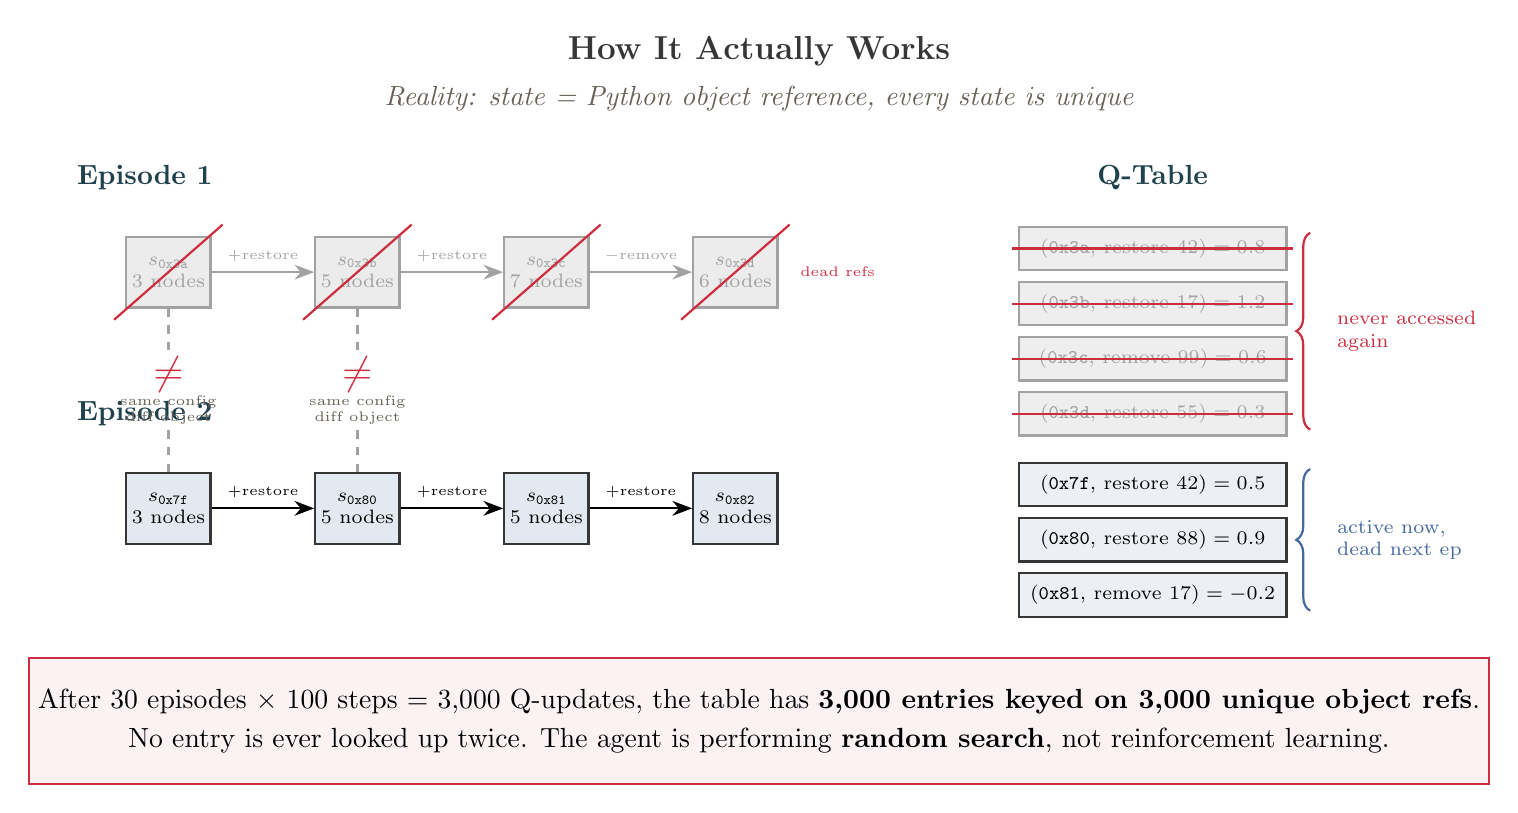
\begin{tikzpicture}[
    every node/.style={font=\small},
    state/.style={draw=Black90, thick, minimum size=0.9cm, inner sep=2pt,
        align=center, font=\scriptsize},
    deadstate/.style={draw=Black50, thick, minimum size=0.9cm, inner sep=2pt,
        align=center, font=\scriptsize, text=Black50},
    qtable/.style={draw=Black90, thick, minimum width=3.4cm, minimum height=0.55cm,
        align=center, font=\scriptsize},
    deadq/.style={draw=Black50, thick, minimum width=3.4cm, minimum height=0.55cm,
        align=center, font=\scriptsize, text=Black50, fill=Black30!30},
    arr/.style={-{Stealth[length=2.5mm]}, thick},
    xarr/.style={thick, Rose},
]

% === Title ===
\node[font=\large\bfseries, Black90] at (7.5, 8.8) {How It Actually Works};
\node[font=\normalsize\itshape, WarmGrey] at (7.5, 8.2)
    {Reality: state = Python object reference, every state is unique};

% =============================================
% EPISODE 1
% =============================================
\node[font=\normalsize\bfseries, Congaree] at (-0.3, 7.2) {Episode 1};

\node[deadstate, fill=LightGray] (e1s1) at (0, 6.0) {$s_{\texttt{0x3a}}$\\3 nodes};
\node[deadstate, fill=LightGray] (e1s2) at (2.4, 6.0) {$s_{\texttt{0x3b}}$\\5 nodes};
\node[deadstate, fill=LightGray] (e1s3) at (4.8, 6.0) {$s_{\texttt{0x3c}}$\\7 nodes};
\node[deadstate, fill=LightGray] (e1s4) at (7.2, 6.0) {$s_{\texttt{0x3d}}$\\6 nodes};

\draw[arr, Black50] (e1s1) -- (e1s2) node[midway, above, font=\tiny, Black50] {+restore};
\draw[arr, Black50] (e1s2) -- (e1s3) node[midway, above, font=\tiny, Black50] {+restore};
\draw[arr, Black50] (e1s3) -- (e1s4) node[midway, above, font=\tiny, Black50] {$-$remove};

% Cross out ep1 states
\draw[xarr] ([xshift=-4pt, yshift=-4pt]e1s1.south west) --
    ([xshift=4pt, yshift=4pt]e1s1.north east);
\draw[xarr] ([xshift=-4pt, yshift=-4pt]e1s2.south west) --
    ([xshift=4pt, yshift=4pt]e1s2.north east);
\draw[xarr] ([xshift=-4pt, yshift=-4pt]e1s3.south west) --
    ([xshift=4pt, yshift=4pt]e1s3.north east);
\draw[xarr] ([xshift=-4pt, yshift=-4pt]e1s4.south west) --
    ([xshift=4pt, yshift=4pt]e1s4.north east);

\node[font=\tiny, Rose, anchor=west] at (7.9, 6.0) {dead refs};

% =============================================
% EPISODE 2
% =============================================
\node[font=\normalsize\bfseries, Congaree] at (-0.3, 4.2) {Episode 2};

\node[state, fill=Atlantic!15] (e2s1) at (0, 3.0) {$s_{\texttt{0x7f}}$\\3 nodes};
\node[state, fill=Atlantic!15] (e2s2) at (2.4, 3.0) {$s_{\texttt{0x80}}$\\5 nodes};
\node[state, fill=Atlantic!15] (e2s3) at (4.8, 3.0) {$s_{\texttt{0x81}}$\\5 nodes};
\node[state, fill=Atlantic!15] (e2s4) at (7.2, 3.0) {$s_{\texttt{0x82}}$\\8 nodes};

\draw[arr] (e2s1) -- (e2s2) node[midway, above, font=\tiny] {+restore};
\draw[arr] (e2s2) -- (e2s3) node[midway, above, font=\tiny] {+restore};
\draw[arr] (e2s3) -- (e2s4) node[midway, above, font=\tiny] {+restore};

% =============================================
% NO CONNECTION between episodes
% =============================================
% Attempted dotted line with X
\draw[dashed, Black50, thick] (e1s1.south) -- ++(0, -0.6);
\draw[dashed, Black50, thick] (e2s1.north) -- ++(0, 0.6);
\node[font=\Large\bfseries, Rose] at (0, 4.7) {$\neq$};
\node[font=\tiny, WarmGrey, align=center] at (0, 4.25) {same config\\diff object};

\draw[dashed, Black50, thick] (e1s2.south) -- ++(0, -0.6);
\draw[dashed, Black50, thick] (e2s2.north) -- ++(0, 0.6);
\node[font=\Large\bfseries, Rose] at (2.4, 4.7) {$\neq$};
\node[font=\tiny, WarmGrey, align=center] at (2.4, 4.25) {same config\\diff object};

% =============================================
% Q-TABLE (shows dead entries)
% =============================================
\node[font=\normalsize\bfseries, Congaree] at (12.5, 7.2) {Q-Table};

% Episode 1 entries (dead)
\node[deadq] (q1) at (12.5, 6.3)
    {$(\texttt{0x3a}$, restore 42$) = 0.8$};
\node[deadq] (q2) at (12.5, 5.6)
    {$(\texttt{0x3b}$, restore 17$) = 1.2$};
\node[deadq] (q3) at (12.5, 4.9)
    {$(\texttt{0x3c}$, remove 99$) = 0.6$};
\node[deadq] (q4) at (12.5, 4.2)
    {$(\texttt{0x3d}$, restore 55$) = 0.3$};

% Cross out dead entries
\draw[xarr] ([xshift=-2pt]q1.west) -- ([xshift=2pt]q1.east);
\draw[xarr] ([xshift=-2pt]q2.west) -- ([xshift=2pt]q2.east);
\draw[xarr] ([xshift=-2pt]q3.west) -- ([xshift=2pt]q3.east);
\draw[xarr] ([xshift=-2pt]q4.west) -- ([xshift=2pt]q4.east);

% Episode 2 entries (active but also doomed)
\node[qtable, fill=Atlantic!10] (q5) at (12.5, 3.3)
    {$(\texttt{0x7f}$, restore 42$) = 0.5$};
\node[qtable, fill=Atlantic!10] (q6) at (12.5, 2.6)
    {$(\texttt{0x80}$, restore 88$) = 0.9$};
\node[qtable, fill=Atlantic!10] (q7) at (12.5, 1.9)
    {$(\texttt{0x81}$, remove 17$) = -0.2$};

% Braces
\draw[decorate, decoration={brace, amplitude=5pt, mirror}, thick, Rose]
    (14.5, 6.5) -- (14.5, 4.0)
    node[midway, right=6pt, font=\scriptsize, text=Rose, align=left]
    {never accessed\\again};

\draw[decorate, decoration={brace, amplitude=5pt, mirror}, thick, Atlantic]
    (14.5, 3.5) -- (14.5, 1.7)
    node[midway, right=6pt, font=\scriptsize, text=Atlantic, align=left]
    {active now,\\dead next ep};

% =============================================
% BOTTOM: the real picture
% =============================================
\node[draw=Rose, thick, fill=Rose!6, minimum width=14.5cm,
    minimum height=1.6cm, align=center, font=\normalsize] at (7.5, 0.3)
    {After 30 episodes $\times$ 100 steps = 3{,}000 Q-updates, the table has
    \textbf{3{,}000 entries keyed on 3{,}000 unique object refs}.\\[2pt]
    No entry is ever looked up twice.
    The agent is performing \textbf{random search}, not reinforcement learning.};

\end{tikzpicture}
\end{document}
